\documentclass[../main/main.tex]{subfiles}
\begin{document}


\chapter{Un spectrographe 3D: La Spectral Energy Distribution machine}\label{ch:sedm}

\minitoc
\vspace{2cm}
Dans le chapitre précédent, nous avons présenté la collaboration Zwicky
Transient Facility et nous nous sommes focalisés sur la caméra
principale de $47\text{deg}^{2}$ montée sur le P48 au Mont
Palomar. Cette caméra permet à ZTF de détecter $10^{5}$ évènements
transitoires ou variables, en scannant l'entièreté du ciel Nord visible
chaque nuit,  à la vitesse
vertigineuse de $3760\text{deg}^{2}$/heure. Parmi ces évènements,
$\mathcal{O}(10)$ correspondent à de nouveux évènements transitoires non
répertoriés: Les Supernovae. Comme expliqué dans le
Chapitre~\ref{sec:snia}, seules les Supernovae de type Ia sont
d'intérêts dans la cosmologie, de part leur propriété de chandelle
standardisable. Il faut donc les classifier. Pour cela, on utilise leur
spectre, dont les raies d'absorbtion/émission sont caractéristiques d'un
type à l'autre de SN. Ainsi, ZTF possède également un spectrographe 3D
monté sur le télescope P60 au Mont Palomar
(Figure~\ref{fig:palomar_obs}) spécialement conçu à cet effet. Nous
présentons dans ce chapitre ce spectrographe, la Spectral Energy
Distribution machine (SEDm).
\newpage

\section{Présentation de l'instrument}
\label{sec:ifs}

\subsection{Principe d'un IFS}
Le spectrographe 3D SEDm est ce qu'on appelle un IFS pour Integral Field
Spectrograph. Sans surprise, c'est un instrument qui permet de
recueillir le spectre du ciel sur un champ de vue bidimensionnel.
Ainsi et indépendamment de la méthode utilisée, le produit final avec
cet instrument correspond à
un cube de données ayant 2 dimensions spatiales (($x$, $y$) ou (RA,
Dec) ) et une dimension spectrale (longueur d'onde $\lambda$ ou une
vitesse).

Un IFS est composé de 2 parties: le spectrographe qui va disperser la
lumière incidente, et l'IFU (Integrated Field Unit). Le rôle de l'IFU
est de diviser le plan spatial 2D du champ de vue en réseau continue
et concentré de lumière. Ce réseau est ensuite donné en entrée au
spectrographe qui va se charger de le disperser sur le détecteur.

Il existe 3 types principaux d'IFU, schématisés dans la Figure~\ref{fig:ifsgeneral}.
\begin{itemize}[label=$\bullet$]
\itemsep0em 
\item \textbf{Le réseau de micro-lentilles} conceptualisé par
  \citet{BaconIFUlens} (qui s'apparente aux yeux composites
  de certains insectes): C'est le système utilisé par la SEDm, mais
  également par l'IFS SAURON \citep{SAURONifs} dans le projet ATLAS3D
  \citep{ATLAS3D} ou encore SNIFS \citep{SNIFS2004}. Dans ce système,
  l'image bi-dimensionnelle est fractionnée par un réseau de
  micro-lentilles (le MLA, microlens array). Chaque élément est ensuite
  concentré et dispersé par le spetrographe (voir
  Figure~\ref{fig:ifsgeneral}). Pour éviter au maximum le chevauchement des
  spectres sur le détecteur, le réseau de lentille est légèrement
  incliné. Le désavantage principal de cette technique est le court
  intervalle de longueur d'onde dispersable sans induire de chevauchement.
  
\item \textbf{Le paquet de fibre} comme
  avec l'IFS du relevé MaNGA d'SDSS \citep{SDSSIFS} qui peut
  être utilisé en combinaison \citep{BardenIFUfiber} ou non
  \citep{allingtonIFUlensfiber} de réseau de micro-lentilles.
  Ici la lumière n'est pas concentrée par des lentilles mais acheminée
  par un paquet de fibres optiques ``à la chaîne'' jusqu'à la fente du spectrographe. Le
  premier avantage est bien évidemment la flexibilité des fibres. Mais
  en contrepartie l'échantillon du ciel disperé devient non contigu, à
  cause de la forme circulaire des fibres. Il est possible de pallier à
  cet effet un ajoutant un réseau de micro-lentilles (lui contigu) entre
  le plan focal et le paquet de fibres.  
  
\item \textbf{Le ``trancheur d'image''} qui est la méthode la plus
  ancienne (\citet{BowenIFUslicer}, \citet{ContentIFUslicer}) utilisée
  par exemple avec le NIFS
  (near-infrared integral field spectrograph, \citet{GeminiNIFS}). Cette
  méthode utilise un mirroir segmenté en fines sections
  horizontales. Chacune de ces sections va diriger la lumière incidente
  dans des directions légèrement différentes jusqu'à un second miroir
  segmenté. Ce dernier va réarranger les tranches incidentes non pas
  l'une au dessus de l'autre, mais de façon étalées, ``à la chaîne''
  comme avec la méthode fibrée. L'agencement est ensuite dispersé par la
  fente du spectrographe. Cette méthode permet de conserver la
  contiguïté du champ de vue, mais est en contrepartie couteuse et
  difficile à concevoir.
\end{itemize}

\begin{figure}[h]
  \centering
  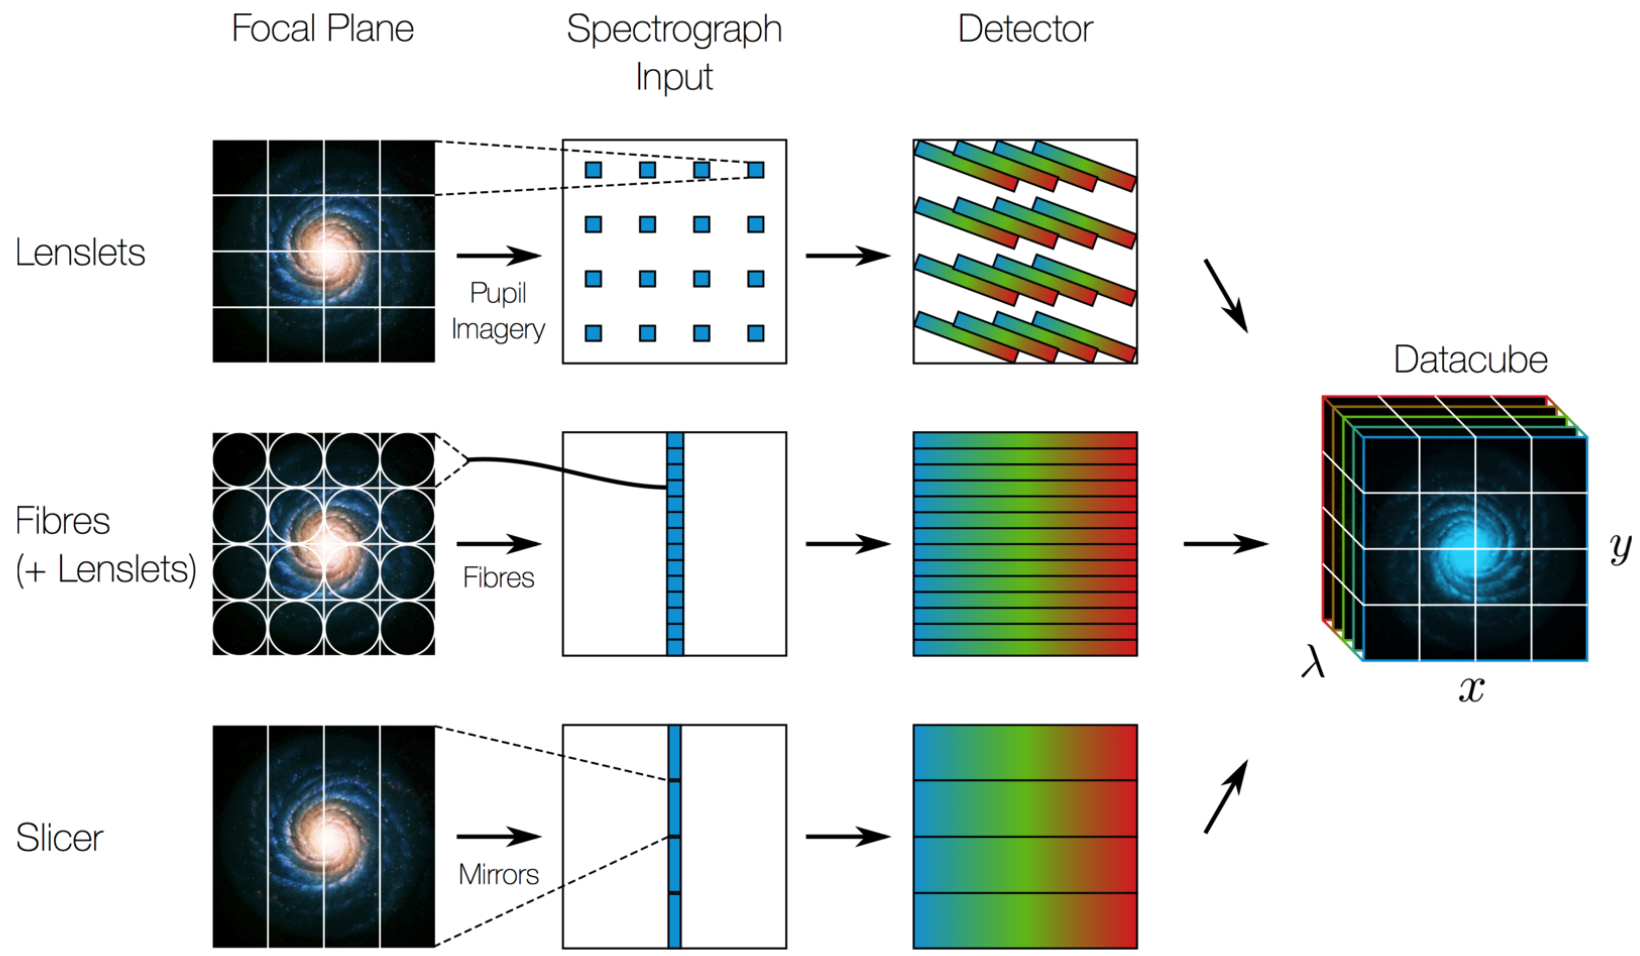
\includegraphics[width=0.9\textwidth]{../figures/03_sedm/ifsgeneral.png}
  \caption[Fonctionnement d'un IFS]{Fonctionnement d'un IFS pour
    différents types d'IFU. La SEDm utilise un système d'agencement de micro-lentilles (cas
    du \textit{haut})
    (\textit{Crédit M. Westmoquette, adaptée de \citet{allingtonIFS}})}
  \label{fig:ifsgeneral}
\end{figure}

Les données brutes obtenues à partir d'un IFS sont ainsi sous la forme
de multiples spectres (de plusieurs dizaines à plusieurs milliers)
étalés (la trace) sur le détecteur, chacun ayant pour origine un élément individuel
de l'IFU. Ces éléments sont en quelques sortes des pixels spatiaux, que
l'on contracte communément par le terme de spaxels. La reconstruction du
cube de données se fait en extrayant chaque spectre du détecteur, et en
les réarrangeant dans le même espace géométrique que le plan focal du
télescope (nous détaillerons ce processus dans la section suivante).

\subsection{La SEDm}

Focalisons nous maintenant sur notre instrument, la Spectral Energy
Distribution machine, présenté par \citet{SEDM18}. Comme mentionné plusieurs fois, celui ci est monté
sur le télescope P60 (Cassegrain) au Mont Palomar depuis Août 2016. Une vue
d'ensemble de l'instrument est présenté dans la
Figure~\ref{fig:sedmoverview}, où l'on peut voir qu'il est composé de
deux canaux: l'IFU et la ``Rainbow Camera'' (RC), montés sur un
agencement en forme de T. Cette caméra d'acquisition multi-bande est
accompagnée de 4 filtres photométriques $u'$, $g'$, $r'$ et $i'$.


\begin{figure}[h]
  \centering
  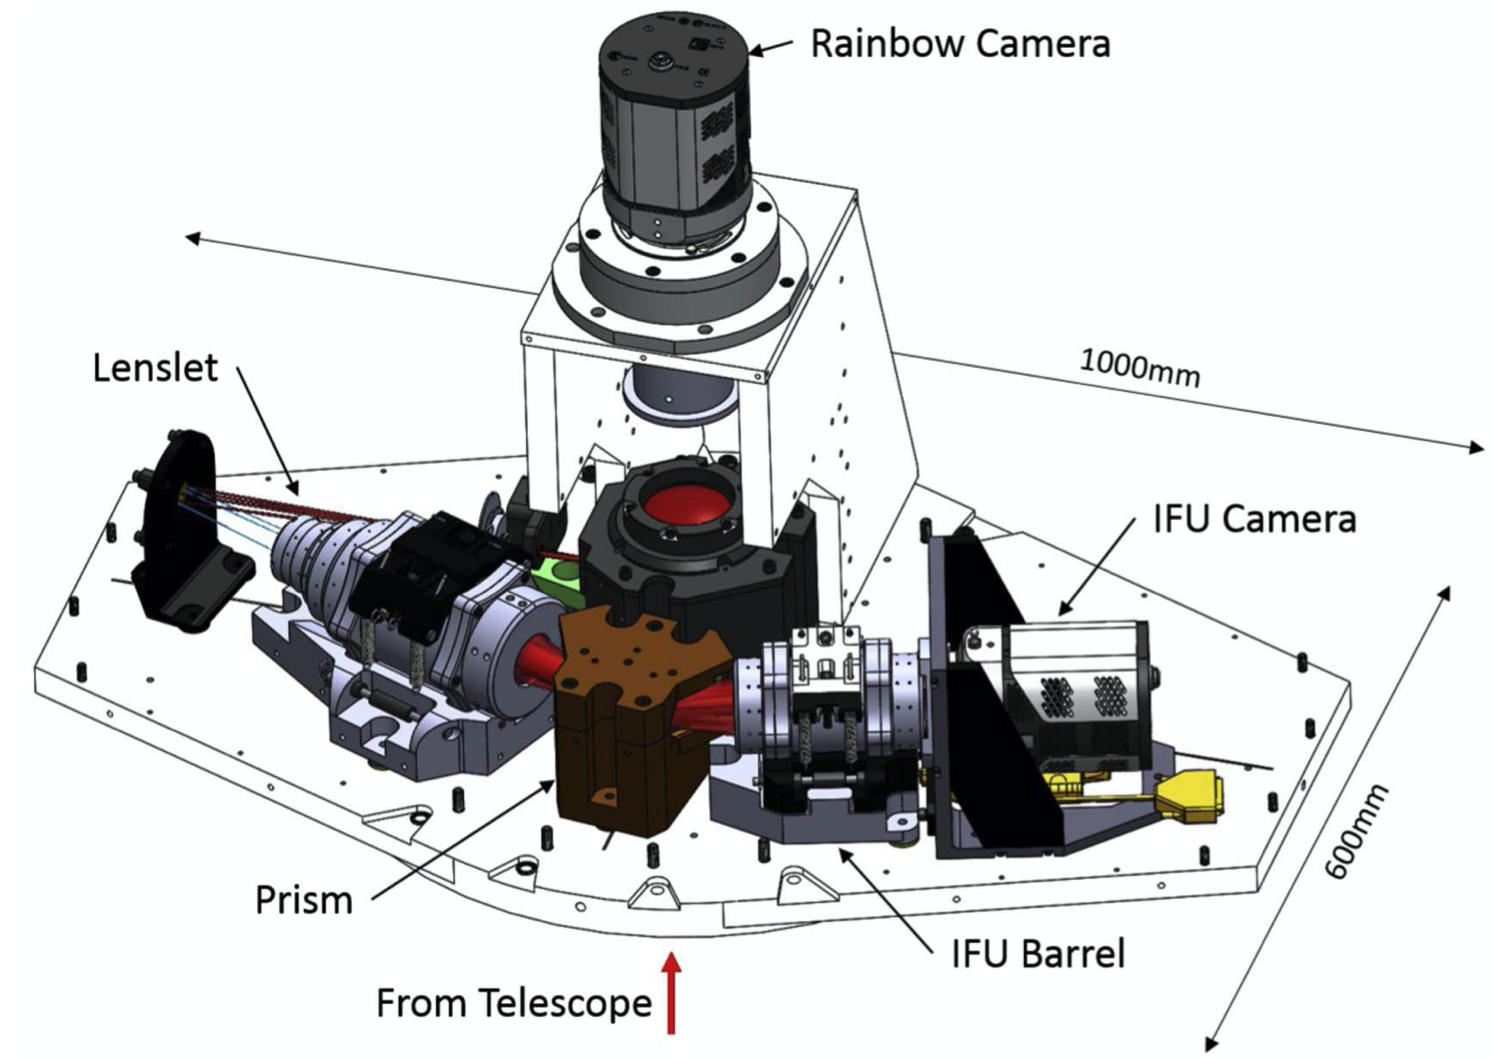
\includegraphics[width=0.9\textwidth]{../figures/03_sedm/sedmoverview.png}
  \caption[Vue d'ensemble de la SEDm]{Vue d'ensemble de la SEDm
    \citep{SEDM18}. La source de lumière du Cassegrain est indiqué par
    la lumière rouge. L'instrument photométrique, la RC, est situé en
    haut au centre et récolte directement la lumière. Pour l'IFU, la
    lumière est redirigée jusqu'à un miroir que l'on peut voir tout à
    gauche de la représentation. Elle est ensuite réfléchie dans le MLA
    (Lenslet). La lumière de chaque micro-lentille du MLA passe ensuite
    dans le prisme (en marron au centre) pour y être dispersé et
    focalisé par l'optique (IFU Barrel) sur le détecteur (IFU Camera).}
  \label{fig:sedmoverview}
\end{figure}

Les 2 caméras de la SEDm sont des Princeton Instruments identiques:
une PIXIS 2048B et une PIXIS 2048B\_Excelon chacun avec 2048$\times$2048
pixels de taille \SI{13.5}{\micro\metre}.

La Rainbow Camera est utilisée pour le guidage, la calibration,
l'acquisition de cible ou encore l'imagerie scientifique. Le champ de
vue de $13\arcmin\times13\arcmin$ est divisé en 4 quadrants, un pour
chacun des filtres $u'g'r'i'$.

L'IFU de la SEDm fonctionne sur la méthode du réseau de micro-lentilles,
le MLA. Celui ci couvre un champ de vue de $28\times28\arcsec$, avec
$45\times52$ lentilles hexagonales. Le faisceau de lumière projeté par
ces lentilles passe dans un triple prisme avec une résolution spectrale
achromatique de $R=\frac{\lambda}{\Delta\lambda}\sim100$.
Comme illustré dans la Figure~\ref{fig:sedmoverview}, c'est la RC qui
est alignée avec la lumière directe en provenance du Cassegrain. Il faut donc en dévier une
partie qui sera transmise à la caméra de l'IFU: cela est effectué avec un
prisme d'interception centré sur le faisceau incident, qui va rediriger
le champ de $28\times28\arcsec$ vers un miroir. Les images
photométriques de la RC ont donc en leur centre un masque qui correspond
au champ de vue de l'IFU. Ainsi pour faire l'acquisition d'une cible
avec l'IFU, il faut d'abord effectuer une acquisition avec la RC sur
laquelle un fitter d'astrometrie est appliqué. Cette étape fournie une
information précise sur le pointage du télescope, et permet donc
d'appliquer l'offset nécessaire pour positionner la cible au centre du
champ de vue de l'IFU.

\section{Extraction des spectres du CCD et création des cubes de données}
%\label{ssec:xxx}

\section{Actuelle méthode d'extraction de point source}
%\label{ssec:xxx}

\section{SEDm en quelques chiffres}
%\label{ssec:xxx}

\bibliographystyle{../main/aa_url}
\bibliography{99_references}
\end{document}

%%% Local Variables:
%%% mode: latex
%%% TeX-master: t
%%% End:
